\subsection*{Data acquisition}
We recorded the calcium activity  of dense populations of neurons in the supragranular layers in primary visual cortex of anesthetized mice using fast random-access 3D scanning two-photon microscopy \cite{Stosiek:2003,Reddy:2005}.  Numerious repetitions of full-field drifting gratings (Fig. 1A and 1B) were presented to the eye contralateral to the imaged site. This technique allowed recording from a large number (150--350) of cells in a small volume of cortical tissue ($200\times200\times100$ $\mu$m$^3$) in layers 2/3 and 4. Somatic calcium signals were deconvolved using  sparse nonnegative deconvolution \cite{Vogelstein:2010} (Fig.\;1C and 1D).  The average stimulus response was subtracted to remove stimulus covariance and the sample noise covariance matrix was computed (Fig.\;1E).

\begin{figure}[htp]
\begin{center}
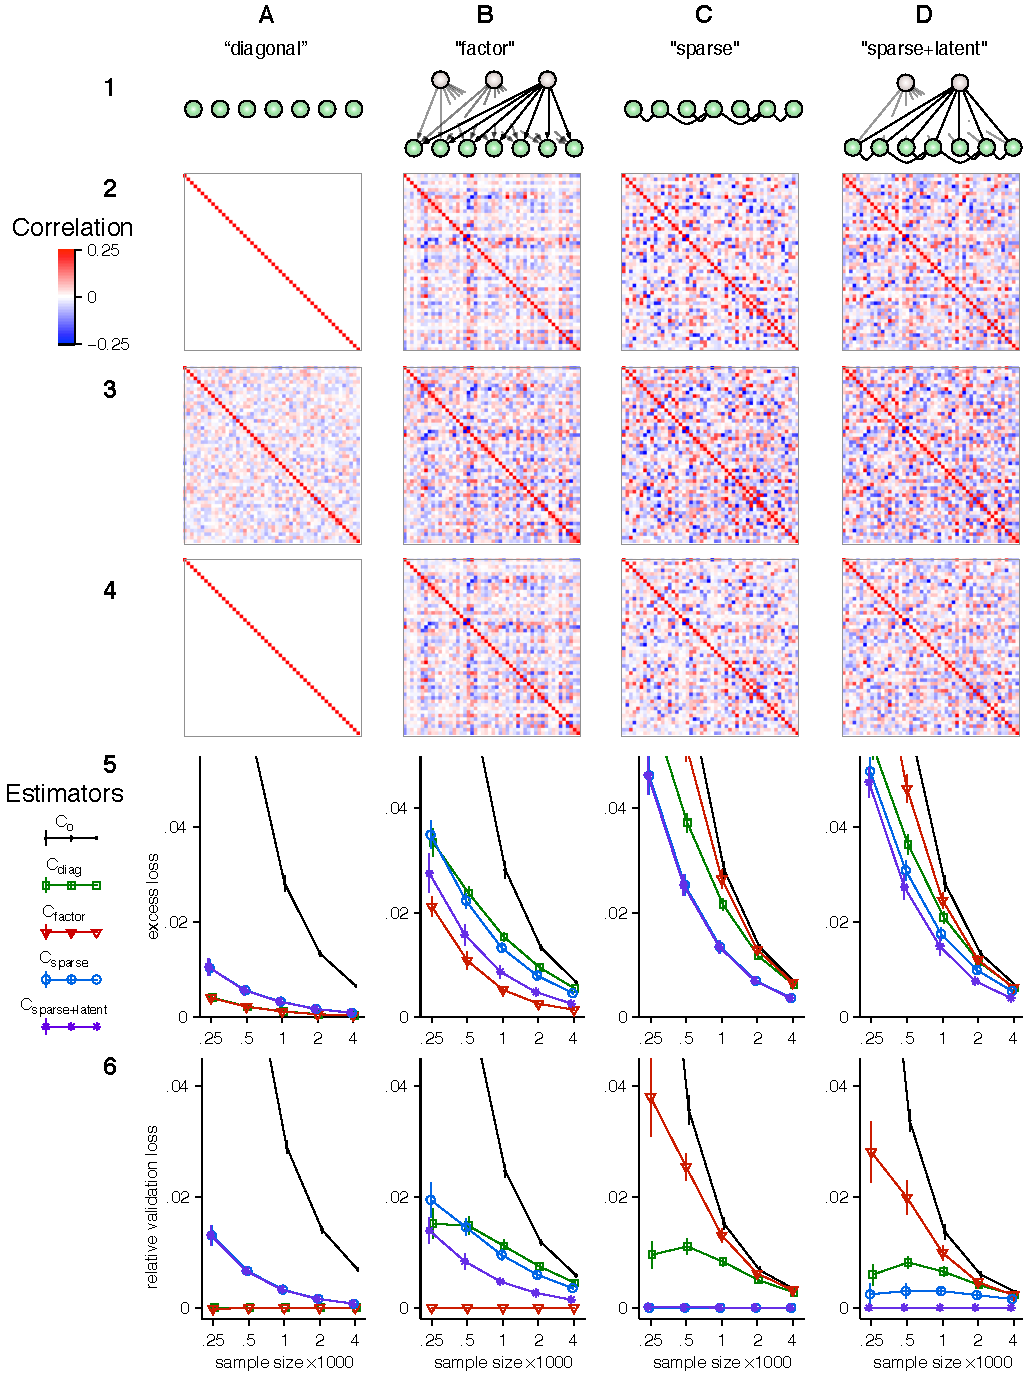
\includegraphics[width=2.5in]{figures/Figure1.pdf}
\end{center}
\caption{
{\bf Acquistion of neural population activity using two-photon fluorescence imaging of calcium signal.}  {\bf A.} Visual stimuli comprising brief (500 ms) presentatios of full-field drifting gratings separated by blank screens. {\bf B.} Two-photon fast 3D imaging of calcium signals in an awake mouse. {\bf C.} Deconvolved calcium signals. {\bf D.} The sample covariance matrix of neuronal calcium signals in 200 ms time bins. 
}
\label{Figure_label}
\end{figure}


\subsection*{The sample covariance matrix}
We aim to estimate the true covariance matrix $\Sigma = \E{(x-\mu)(x-\mu)^\T}$ of the instantaneous activity vector $x$ of a population of $p$ neurons. Here $\E{\cdot}$ denotes expectation \TODO{for the true data generating process} and $x$ is the $p\times 1$ vector of real-valued instantaneous firing rates discretized into bins of duration $\Delta t$ and $\mu = \E{x}$.  

For more rigorous notation, definitions, and derivations, see Appendix. 

The usual estimator of $\Sigma$ is the sample covariance matrix
\begin{equation}
\hat \Sigma_0 = \frac 1 {n-c} \sum\limits_{t=1}^n (x(t)-\mu)(x(t)-\mu)^\T 
\end{equation}
where $x(t),\;t=1,\ldots,n$ are sequential observations of population activity inferred from calcium signals. Bessel's correction $c$ makes the estimate unbiased such that $\E{\hat\Sigma_0} = \Sigma$. When observations $x(t)$ can be assumed to be independent then $c=1$; but when observations are correlated $c>1$ may be estimated from the data. 

\subsection*{Evaluation of covariance matrix estimates}
The quality of a covariance matrix estimate $\hat\Sigma$ is measured by a real-valued \emph{loss function} $\loss{\hat\Sigma,\Sigma}$.  The loss function quantifies the deviation of $\hat\Sigma$ from $\Sigma$ and attains its minimum  when $\hat\Sigma = \Sigma$. 

For the purposes of this study, we adopted the \emph{negative normal log-likelihood loss} function:
\begin{equation}\label{eq:loss}
\loss{\hat\Sigma,\Sigma} = \frac 1 p\left[\ln \det \hat \Sigma + \Tr(\hat \Sigma^{-1}\Sigma)\right]
\end{equation}
This choice is motivated by mathematical convenience. Other popular choices for the loss function are the Frobenius norm of the difference $\hat\Sigma-\Sigma$, Stein's entropy loss, and quadratic loss \cite{James:1961,Ledoit:2004,Schafer:2005,Fan:2008}.  We assert that the main conclusions of our study are unlikely to change drastically other well behaved loss functions.

The aim of our project is produce covariance matrix estimates that minimize the expected loss.  The expected loss of an estimator is known as its \emph{risk}: 
\begin{equation}
r = \E{\loss{\hat\Sigma, \Sigma}}
\end{equation}

In practice, the true value $\Sigma$ is not accessible and estimators' risks must be estimated from the data.  This may be accomplished through validation: 
Let $\hat\Sigma_0^\prime$ denote a sample covariance matrix measured from an independent sample that was not used included in the computation of $\hat\Sigma$. Then \emph{empirical loss} is 
\begin{equation}
\hat \ell = \loss{\hat\Sigma,\hat\Sigma_0^\prime}
\end{equation}
 and its expected value or \emph{empirical risk} is
\begin{equation}\label{eq:empiricalRisk}
\hat r = \E{\hat\ell} = \mathbb E_{\hat\Sigma} \left[ \mathbb E_{\hat\Sigma_0^\prime} \left[ {\loss{\hat\Sigma,\hat\Sigma_0^\prime}} \right] \right]
\end{equation}
Because the chosen loss function is linear in its second argument in the sense that
\begin{equation}
\loss{\hat\Sigma,X_1} + \loss{\hat\Sigma,X_2} \equiv \loss{\hat\Sigma,X_1+X_2}
\end{equation}
the expection on the second argument in Eq.~\ref{eq:empiricalRisk} may be taken inside the loss function:
\begin{equation}
\hat r = \E{\loss{\hat\Sigma,\E{\hat\Sigma_0^\prime}}}  = \E{\loss{\hat\Sigma,\Sigma}} = r
\end{equation}
Thus the empirical loss $\loss{\hat \Sigma,\hat \Sigma_0^\prime}$ serves as an unbiased estimate of risk $r$. 

Because the loss function is equivalent to the negative normal log likelihood, the above derivation led us to the familiar criterion that the optimal covariance matrix estimator is one that consistently maximizes the normal log likelihood of the validation dataset.

\subsection*{Regularization}
Under many loss functions\footnote{
The strict equality in Eq.~\ref{eq:bias-variance} does not hold under the loss function in Eq.~\ref{eq:loss}. However, the equality does hold for its close cousin, Stein's \emph{entropy loss},  which only differs by the order of its arguments and a constant offset: $\mathcal L_s(\hat\Sigma,\Sigma) \equiv \loss{\Sigma,\hat\Sigma} - \loss{\Sigma,\Sigma}$. This defficiency presents no difficulty because we minimize the risk directly, without assessing the two error components individually. The bias-variance decomposition is presented here to motivate the use of regularization.}, 
the estimator's risk can be decomposed as the sum
\begin{equation}\label{eq:bias-variance}
r = b + \varepsilon
\end{equation}
of \emph{approximation error} (``bias'' or systematic error)
\begin{equation}
b = \loss{\bar\Sigma,\Sigma}
\end{equation}
and \emph{estimation error} (``variance'') 
\begin{equation}
\varepsilon = \E{\loss{\hat\Sigma, \bar\Sigma}}
\end{equation}
where $\bar\Sigma = \E{\hat\Sigma}$ is the expected value of the estimate. 

The unbiased estimator $\hat\Sigma_0$ makes $\bar\Sigma=\Sigma$ and thereby minimizes the approximation error, but may be excessively susceptible to sample noise and result in high estimation error.

The estimator risk can be reduced by \emph{regularization}. Regularization is the deliberate biasing (\emph{``shrinkage''}) of the estimate toward a low-dimensional, less variable \emph{target estimate} \cite{Bickel:2006,Ledoit:2004}. A regularized estimator solves the bias-variance tradeoff to produce a biased but less variable estimates aiming to minimize the estimator's risk.  Various regularization schemes focus on the dimensionality reduction part \TODO{rephrase} by selecting the optimal target estimate from a family of estimates with reduced dimensionality \cite{findit}.  Other estimators only shrink the sample covariance matrix toward a single target estimator \cite{Schafer:2005}. Yet other regularizers effectively combine shrinkage and dimensionality reduction \cite{findit}.

We evaluated four regularized estimators denoted here as A, B, C, and D.  Their target estimates correspond to covariance matrices of Gaussian graphical models depicted in Figure 2 where green spheres represent the recorded neurons,  light-colored spheres represent latent units of the graphical model, and edges connecting them represent conditional dependencies or interactions.

\begin{figure}[htp]
\centering
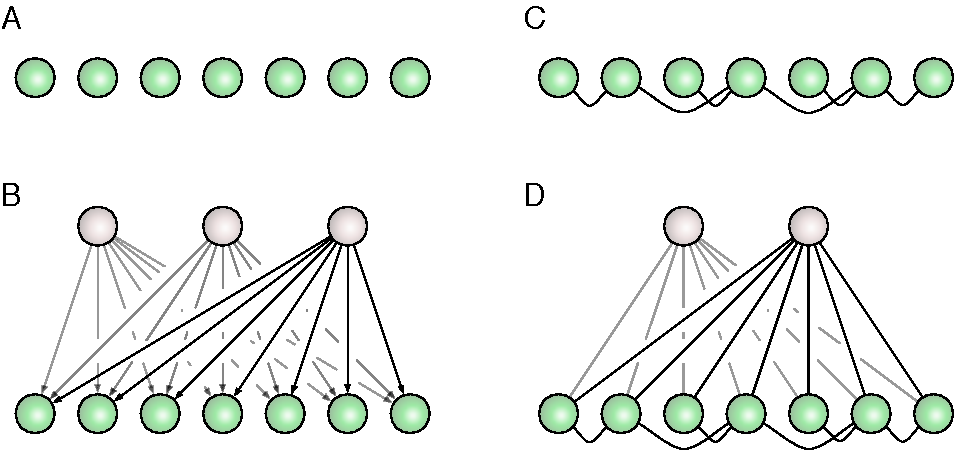
\includegraphics[width=0.5\textwidth]{figures/Figure2.pdf}
\caption{
Graphical models corresponding to the low-dimensional targets of the four regularization schemes used in the paper.
\textbf{A}: A diagonal matrix corresponds to a Gaussian graphical model with no dependencies.
\textbf{B}: In factor analysis, observed nodes are assumed to be influenced by several latent units (``factors") but are otherwise independent.
\textbf{C}: Graphical model with conditional dependencies between a specified subset of pairs of observed neurons, no latent units. 
\textbf{D}: Graphical model with conditional dependencies between a specified subset of pairs of observed neurons and dense interactions with a few latent units.
}\label{fig:02}
\end{figure}


A \emph{graphical model} is a multivarate probability distribution with a specified graph of conditional dependencies between its variables \cite{Koller:2009}.  When this distribution is a multivariate normal distribution, the model becomes a \emph{Gaussian graphical model} (GGM) or, equivalently, a \emph{Gaussian Markov Random Field}.  Gaussian graphical models have a straightforward relationship to their covariance matrix $\Sigma$:  Zero elements in the inverse of $\Sigma$ indicate conditional independence between the corresponding pair of variables.  

Fitting a graphical model to data involves two tasks: (1) the selection of the set of non-zero covariances or \emph{covariance selection} \cite{Dempster:1972} and (b) the fitting of the non-zero elements.

\subsubsection*{Estimator A: Shrinkage toward identity.}
In \emph{estimator A}, the sample covariance matrix $\hat\Sigma_0$ is shrunk toward the independent model.  The covariance matrix of a GGM in which all units are independent will be diagonal.  
For example, we  could leave the sample variances on the diagonal and zero out the off-diagonal products, making the target estimate 
\begin{equation}\label{eq:sampleVariance}
\hat T= \hat\Sigma_0\circ I
\end{equation}
where $\circ$ denotes the entrywise matrix product (Hadamard product). 
Alternatively, the target could have equal variances, all equal to the average sample variance in the population $v = \frac 1 p \Tr(\hat\Sigma_0)$.
\begin{equation}\label{eq:equalVariance}
\hat T=\frac 1 p \Tr(\hat\Sigma_0) I
\end{equation}
The equal-variance target in Eq.~\ref{eq:equalVariance} has only one degree of freedom and thus lower estimation error but higher bias than the target with sample variances in Eq.~\ref{eq:sampleVariance}. It is not immediately clear which target is better in a particular application. We therefore use the linear mixture of the two targets paramaterized by the mixing coefficient $\alpha\in[0,1]$:
\begin{equation}
\hat T_\alpha = (1-\alpha)(\hat\Sigma_0 \circ I) + \frac \alpha p \mbox{tr}(\hat \Sigma_0)I
\end{equation}
Then the estimator $\hat\Sigma_{\alpha,\lambda}$ is the linear shrinkage of the sample covariance matrix $\hat\Sigma_0$ toward $\hat T_\alpha$ controlled by the mixing proportion $\lambda\in[0,1]$:
\begin{equation}
\hat\Sigma_{\alpha,\lambda} = (1-\lambda)\hat\Sigma_0 + \lambda\hat T_\alpha 
\end{equation}
This covariance matrix estimator is implemented by R's {\tt corpcor} package \cite{Schaefer:2010} and enjoys widespread use in many applications \cite{Schafer:2005}.

We estimated the optimal values of hyperparameters $ \alpha$ and $ \lambda$  by nested cross-validation within the training dataset. \TODO{more detail?}

\subsubsection*{Estimate B: Shrinkage toward a factor model}
\emph{Estimator B} shrinks the sample covariance matrix $\hat\Sigma_0$ toward a target estimated by \emph{factor analysis}. For multivariate normal distributions, factor analysis estimates a graphical model in which the observed units do not interact directly but are influenced by a small number of common inputs.

The target estimate
\begin{equation}
T_d = L_dL_d^\T + \Psi
\end{equation}
where $L_d$ is the $p\times d$ \emph{loading matrix} and $\Psi$ is a diagonal matrix. 
where $(L_d,\Psi) = \arg\min\limits_{\dot L_d,\dot\Psi} \loss{\hat\Sigma_0,\dot L_d \dot L_d^\T + \dot \Psi}$ 



 $ \hat T_d$ with $ d$ latent units. When all dependencies are linear, factor models correspond to mutually independent neurons each influenced by $ d$ latent units. (This is  the conventional factor analysis).

Just as in A, the overall estimate is found by linear mixing:
\begin{equation}
\hat\Sigma = (1-\lambda)\hat\Sigma_0 + \lambda\hat T_d
\end{equation}

\subsubsection*{Estimate C}
In estimate C, the target $ \hat S_\alpha$ is a matrix whose inverse is \emph{sparse}, with a large fraction of off-diagonal elements fixed at zero. The coefficient $ \alpha$ controls the sparsity in $ \hat S_\alpha$.

In models with only linear dependencies, zeros in the inverse covariance indicate conditional independence. Thus the target estimate is depicted as the graphical model with sparse interneuronal interactions.

In practice the target $\hat S_\alpha$ is found by an $ L_1$-norm optimization technique, which combines dimensionality reduction and shrinkage into a single computationally efficient algorithm.

Just as in the previous estimators, the optimal value of the regularization parameter $ \alpha$ is determined from the data by nested cross-validation.

\subsubsection*{Estimate D}
In estimate D, the target $\hat R_{d,\alpha}$ is the matrix whose inverse is the sum of a sparse matrix $\hat S_\alpha$ and a low-rank matrix $\hat L_d$ of rank $d$.
\begin{equation}
\hat R_{d,\alpha} = (\hat S_\alpha + \hat L_d)^{-1}
\end{equation}

If all dependencies are linear, the estimate D describes a group of neurons where each interacts with a small number of latent units and a small fraction of the observed neurons. 

\subsection*{Sparse inverse covariance with a low-rank component dominates other estimators}
I computed noise covariances of population activity from 31 sites.  In each site, I compared the cross-validated performance of the covariance matrix using the Gaussian log-likelihood loss function between the trained estimate $ \hat\Sigma$ and the testing sample covariance $ \Sigma_0^\prime$:
\begin{equation}
\mathcal L(\hat\Sigma,\hat\Sigma_0^\prime) = 
\frac 1 p\left( \ln \det \hat \Sigma + \mbox{tr}(\hat \Sigma^{-1}\hat\Sigma_0^\prime) \right) 
\end{equation}

I obtained the following in figure 3.

This is the full matrix of all comparisons of the estimators.  The plots represents the histograms of the differences of the loss function between the pair of estimators for all 31 sites.  When the differences are positive, the first estimate in the title outperforms the second estimate.

Of particular interest is the first row, which shows that all regularized estimates  outperformed the sample covariance estimate.  Even more informative is the last column, which shows that estimate D (sparse+lowrank) significantly outperformed all other estimates.



